\section{Introduction} \label{sec:introduction}
    \IEEEPARstart{R}{espiratory} motion reduces image resolution in \gls{PET} by introducing blurring and mis-alignment artefacts~\cite{Nehmeh2008a}. 

\section{Methods} \label{sec:methods}
    
    
    \subsection{Evaluation} \label{sec:evaluation}
        

\section{Results} \label{sec:results}
    \begin{table}
        \centering
        \captionsetup{singlelinecheck=false, justification=centering}
        \caption{Comparison of \gls{SUV}\textsubscript{max}, \gls{SUV}\textsubscript{median} and \gls{SUV}\textsubscript{peak} between the \glsed{CCP} using a \gls{CCT} \gls{Mu-Map} volume, \glsed{CCP} using a static \gls{CT} \gls{Mu-Map} volume, new method using the \gls{NAC} \gls{RCM} volume and new method using the \gls{AC} \gls{RCM} volume.}
        
        \resizebox*{1.0\linewidth}{!}
        {
            \begin{tabular}{||c|cccc||}
                \hline
                \textbf{\gls{CC}} & \textbf{Static \gls{PCA}} & \textbf{Moving Window} & \textbf{One \gls{PC}} & \textbf{Joint Method} \\
                \hline
                \textbf{Scan $1$}   & $0.0387$  & $0.486$  & $0.565$  & $0.493$   \\
                \textbf{Scan $2$}   & $0.0985$  & $0.0361$ & $0.281$  & $0.0227$  \\
                \textbf{Scan $3$}   & $0.00797$ & $0.0388$ & $0.224$  & $0.00459$ \\
                % \textbf{Scan $4$}   & $0.149$   & $0.0174$ & $0.182$  & $0.0662$ \\
                \textbf{Scan $4$}   & $0.242$   & $0.0467$ & $0.273$  & $0.0946$ \\
                \textbf{Scan $5$}   & $0.0759$  & $0.793$  & $0.819$  & $0.798$ \\
                \textbf{Scan $6$}   & $0.0594$  & $0.246$  & $0.363$  & $0.259$ \\
                \textbf{Scan $7$}   & $0.160$   & $0.629$  & $0.203$  & $0.526$ \\
                % \textbf{Scan $9$}   & $0.238$   & $0.280$  & $0.0752$ & $0.164$ \\
                % \textbf{Scan $10$}  & $0.0343$  & $0.0674$ & $0.0150$ & $0.0460$ \\
                \hline
            \end{tabular}
        }
        \label{tab:cross_correlation}
    \end{table}
    
    \begin{figure}
        \centering
        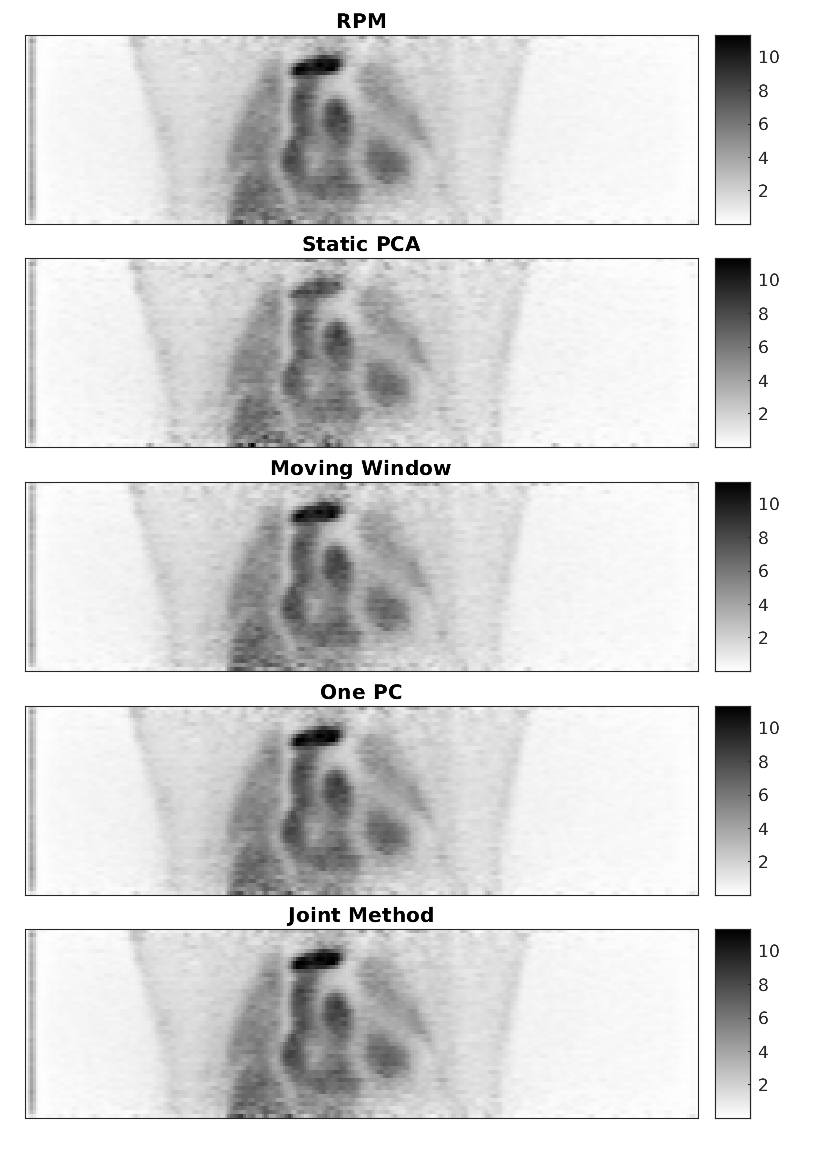
\includegraphics[width=1.0\linewidth]{figures/visual_analysis_pca.png}
        \captionsetup{singlelinecheck=false, justification=centering}
        \caption{First row: \glsed{CCP} using a \gls{CCT} \gls{Mu-Map}. Second row: \glsed{CCP} using a static \gls{CT} \gls{Mu-Map}. Third row: New method using the \gls{NAC} \gls{RCM}. Forth row: New method using the \gls{AC} \gls{RCM}. Colour map ranges are consistent for all images.}
        \label{fig:visual_analysis}
    \end{figure}
    
    \begin{figure}
        \centering
        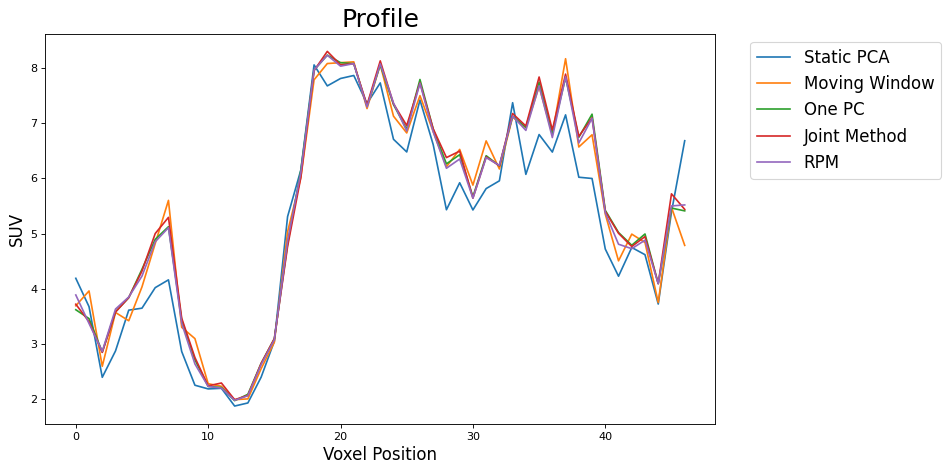
\includegraphics[width=0.5\linewidth]{figures/profile_pca.png}
        \captionsetup{singlelinecheck=false, justification=centering}
        \caption{A profile across the lesion for the \glsed{CCP} using a \gls{CCT} \gls{Mu-Map} volume, \glsed{CCP} using a static \gls{CT} \gls{Mu-Map} volume, new method using the \gls{NAC} \gls{RCM} volume and new method using the \gls{AC} \gls{RCM} volume.}
        \label{fig:profile}
    \end{figure}
    
    \begin{table}
        \centering
        \captionsetup{singlelinecheck=false, justification=centering}
        \caption{Comparison of \gls{SUV}\textsubscript{max}, \gls{SUV}\textsubscript{median} and \gls{SUV}\textsubscript{peak} between the \glsed{CCP} using a \gls{CCT} \gls{Mu-Map} volume, \glsed{CCP} using a static \gls{CT} \gls{Mu-Map} volume, new method using the \gls{NAC} \gls{RCM} volume and new method using the \gls{AC} \gls{RCM} volume.}
        
        \resizebox*{1.0\linewidth}{!}
        {
            \begin{tabular}{||c|ccc||}
                \hline
                \textbf{\gls{SUV}} & \textbf{Max} & \textbf{Median} & \textbf{Peak} \\
                \hline
                \textbf{\gls{RPM}}          & $18.4$ & $10.9$ & $12.6$ \\
                \hline
                \textbf{Static \gls{PCA}}   & $12.8$ & $10.6$ & $11.4$ \\
                \textbf{Moving Window}      & $14.5$ & $10.6$ & $11.3$ \\
                \textbf{One \gls{PC}}       & $18.5$ & $10.9$ & $12.6$ \\
                \textbf{Joint Method}       & $18.5$ & $11.0$ & $12.8$ \\
                \hline
            \end{tabular}
        }
        \label{tab:suv}
    \end{table}
    
     

\section{Discussion and Conclusions} \label{sec:discussion_and_conclusions}
    